\let\negmedspace\undefined
\let\negthickspace\undefined
\documentclass[journal]{IEEEtran}
\usepackage[a5paper, margin=10mm, onecolumn]{geometry}
%\usepackage{lmodern} % Ensure lmodern is loaded for pdflatex
\usepackage{tfrupee} % Include tfrupee package

\setlength{\headheight}{1cm} % Set the height of the header box
\setlength{\headsep}{0mm}     % Set the distance between the header box and the top of the text

\usepackage{gvv-book}
\usepackage{gvv}
\usepackage{cite}
\usepackage{amsmath,amssymb,amsfonts,amsthm}
\usepackage{algorithmic}
\usepackage{graphicx}
\usepackage{textcomp}
\usepackage{xcolor}
\usepackage{txfonts}
\usepackage{listings}
\usepackage{enumitem}
\usepackage{mathtools}
\usepackage{gensymb}
\usepackage{comment}
\usepackage[breaklinks=true]{hyperref}
\usepackage{tkz-euclide} 
\usepackage{listings}
% \usepackage{gvv}                                        
\def\inputGnumericTable{}                                 
\usepackage[latin1]{inputenc}                                
\usepackage{color}                                            
\usepackage{array}                                            
\usepackage{longtable}                                       
\usepackage{calc}                                             
\usepackage{multirow}                                         
\usepackage{hhline}                                           
\usepackage{ifthen}                                           
\usepackage{lscape}
\begin{document}

\bibliographystyle{IEEEtran}
\vspace{3cm}

\title{NCERT-9.3.11}
\author{EE24BTECH11023 - RASAGNA}

% \maketitle
% \newpage
% \bigskip
{\let\newpage\relax\maketitle}

\renewcommand{\thefigure}{\theenumi}
\renewcommand{\thetable}{\theenumi}
\setlength{\intextsep}{10pt} % Space between text and floats


\numberwithin{equation}{enumi}
\numberwithin{figure}{enumi}
\renewcommand{\thetable}{\theenumi}
\textbf{Question:}

Find the solution of the following differential equation:
$$
(x^3 + x^2 + x + 1) \frac{d}{dx}(y) = 2x^2 + x
$$
\begin{center}
    Given that $x = 0$ when $y = 1$.
\end{center}

\textbf{Solution:}
From the question, after simplification:
$$
\frac{dy}{dx}= \frac{2x^2 + x}{(1+x)(1+x^2)}
$$
Let,
$$
\frac{2x^2 + x}{(1+x)(1+x^2)} = \frac{A}{1+x} + \frac{Bx+C}{1+x^2}
$$
When $x = 0$:
$$
A + C = 0 \quad \text{(eq 1)}
$$
When $x = 1$:
$$
A + B + C = \frac{3}{2} \quad \text{(eq 2)}
$$
When $x = \frac{-1}{2}$:
$$
5A -B + 2C = 0 \quad \text{(eq 3)}
$$
Solving these equations,
$$
A = \frac{1}{2}, \quad B = \frac{3}{2}, \quad C = -\frac{1}{2}
$$
$$
\therefore \frac{dy}{dx} = \frac{1}{2(1+x)} + \frac{3x-1}{2(1+x^2)}
$$
Integrating both sides:
$$
y = \int \left(\frac{1}{2(1+x)} + \frac{3x}{2(1+x^2)} - \frac{1}{2(1+x^2)}\right) dx
$$
The solution is,
$$
y = \frac{1}{2} \ln(1+x) + \frac{3}{4} \ln(1+x^2) - \frac{1}{2} \tan^{-1}(x) + C
$$
Given $x = 0$ when $y = 1$, solve for $C$;
$$
C = 1 - \left(\frac{1}{2} \ln(1+0) + \frac{3}{4} \ln(1+0^2) - \frac{1}{2} \tan^{-1}(0)\right)
$$
$$
\therefore C = 1
$$
Thus, the final required equation is,
$$
y = \frac{1}{2} \ln(1+x) + \frac{3}{4} \ln(1+x^2) - \frac{1}{2} \tan^{-1}(x) + 1
$$
\textbf{Logic for writing the code}
\\
The slope of a tangent at a point $(x_0, y_0)$ on the curve is: 
\[
\frac{dy}{dx} = \lim_{h \to 0} \frac{f(x_0 + h) - f(x_0)}{h}
\]
By moving infinitesimally small distance(h) along the tangent , we get another point $(x_1, y_1)$ .the value of $(x_1,y_1)$
$$
x_1=x_0+h
$$
$$
y_1=y_0+h{\frac{dy}{dx}}
$$
Here, $\frac{dy}{dx} \bigg|_{(x_0, y_0)}$ is the slope at point $(x_0, y_0)$. 
By substituting the values, we obtain $(x_1, y_1)$. 
\\
Similarly, 
\[
x_2= x_1 + h
\]
\[
y_2=y_1+h{\frac{dx}{dy}}
\]
here,
$\frac{dy}{dx} \bigg|_{(x_1, y_1)}$ is the slope at point $(x_1, y_1)$.
Similarly we can obtain n number of points where $$x_n=x_{n-1}+h$$ and $$y_n=y_{n-1}+h{\frac{dy}{dx} \bigg|_{(x_{n-1},y_{n-1})}}$$
 Together these points form the curve representing one of the general solutions of the given Differential Equation. The plot is generated by choosing a known point $(x_0, y_0)$ which satisfies the equation.The value of h is taken to be very small.We generate a large number of points and then plot them.

\section*{PLOTTING THE GRAPH}
\begin{center}
    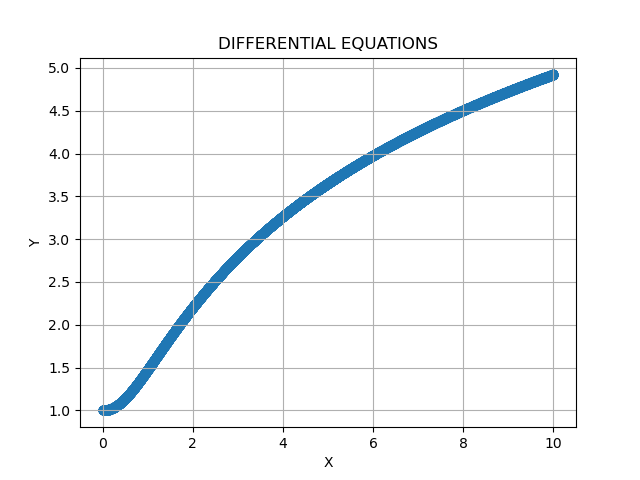
\includegraphics[scale=0.5]{fig/fig.png}
\end{center}

\end{document}